% Fase 3B, exemplos 7–8. Fontes: mb-uso/secoes.
\begin{frame}[fragile]{Exemplo 7 — Em quais regiões a busca chega regularmente?}
\begin{columns}[T,onlytextwidth]
\begin{column}{.39\textwidth}
\textbf{DTLZ2 com 2 objetivos; NSGA-II, 10 execuções.}
\begin{lstlisting}[style=python,basicstyle=\ttfamily\fontsize{7.5}{9.5}\selectfont]
exp1.run(repeat=10)
s01 = mb.stats.attainment(
    exp1, level=0.1)
s05 = mb.stats.attainment(
    exp1, level=0.5)
s09 = mb.stats.attainment(
    exp1, level=0.9)
mb.view.topology(s01,s05,s09)
\end{lstlisting}

\end{column}
\begin{column}{.59\textwidth}
\centering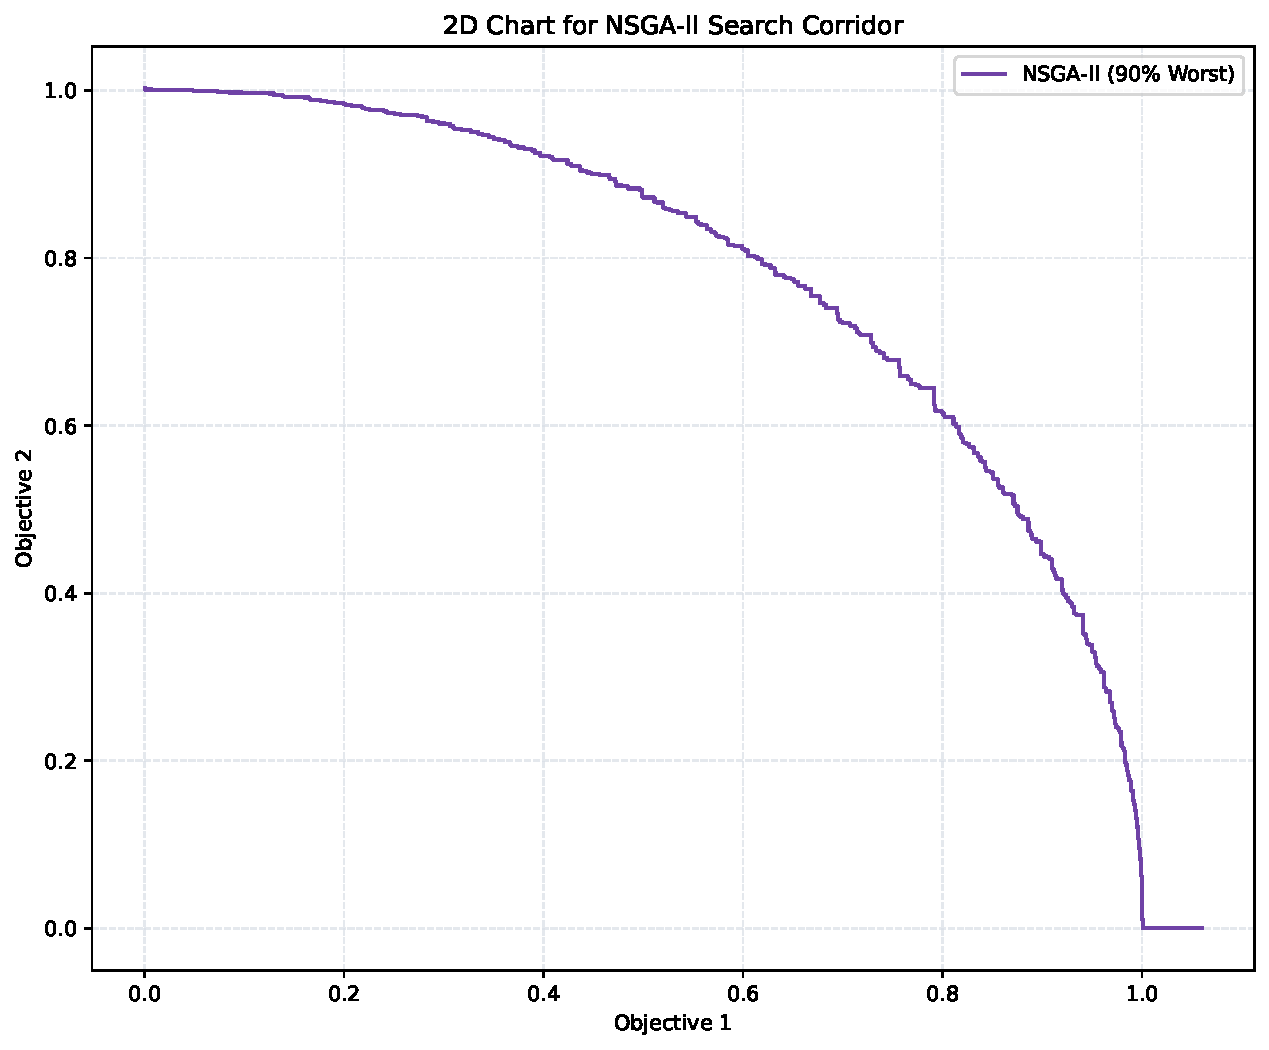
\includegraphics[width=\linewidth,height=.44\textheight,keepaspectratio]{figures/example_07_01_topology.pdf}
\par{\scriptsize Figura original: curva do nível de 90\%; a API também produz 10\% e 50\%.}
\end{column}
\end{columns}
\vspace{.01cm}\textbf{Intuição:} 10\%, 50\% e 90\% são frequências de atingimento, não porcentagens de HV. Regiões atingidas em nove de dez execuções são mais regulares que as atingidas apenas uma vez.
\end{frame}

\begin{frame}[fragile]{Exemplo 7 — Comparar a superfície mediana de dois MOEAs}
\begin{columns}[T,onlytextwidth]
\begin{column}{.61\textwidth}
\centering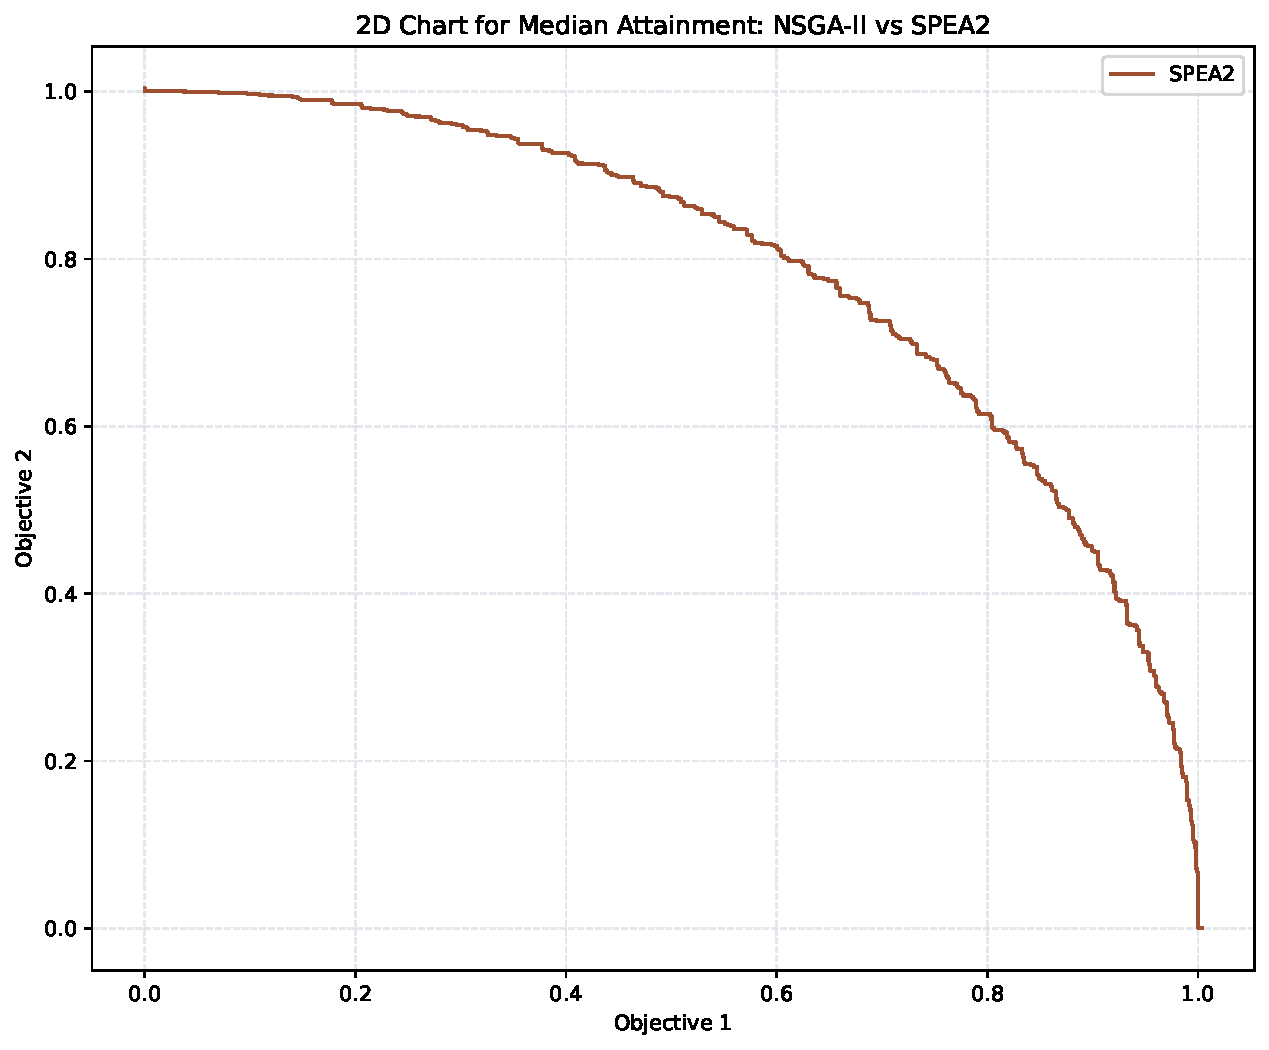
\includegraphics[width=\linewidth,height=.49\textheight,keepaspectratio]{figures/example_07_02_topology.pdf}
\end{column}
\begin{column}{.37\textwidth}
\begin{lstlisting}[style=python,basicstyle=\ttfamily\fontsize{7.4}{9.2}\selectfont]
exp2.run(repeat=10)
gap = mb.stats.attainment_gap(
    exp1, exp2, level=0.5)
gap.report()
mb.view.topology(*gap)
\end{lstlisting}
\textbf{Áreas de atingimento:}
\par NSGA-II: \textbf{0,465884}
\par SPEA2: \textbf{0,421392}
\par Diferença: \textbf{0,044492}
\end{column}
\end{columns}
\vspace{.04cm}\textbf{Interpretação:} no nível mediano de atingimento, NSGA-II cobre região maior. O gráfico também indica \emph{onde} há essa vantagem, informação que uma comparação de HV final pode ocultar.
\end{frame}

\begin{frame}[fragile]{Exemplo 8 — Primeiro: qual o rank de cada solução?}
\textbf{Protocolo:} NSGA-III e SPEA2, dez execuções cada; populações da geração de índice 10.
\begin{columns}[T,onlytextwidth]
\begin{column}{.45\textwidth}
\begin{lstlisting}[style=python,basicstyle=\ttfamily\fontsize{8}{10}\selectfont]
g = 10
ranks = mb.stats.ranks(
    exp1, exp2, gen=g)
\end{lstlisting}
\textbf{Rank 1:} soluções não dominadas no conjunto avaliado.
\par\smallskip
\textbf{Rank 2:} soluções não dominadas após remover as do rank 1; assim sucessivamente.
\end{column}
\begin{column}{.53\textwidth}
\centering
\begin{tikzpicture}[scale=.68]
\draw[->] (0,0)--(6.0,0) node[right]{$f_1$};\draw[->](0,0)--(0,4.8) node[above]{$f_2$};
\foreach \x/\y in {1.0/4,2/2.8,3.6/1.6,5/0.7}{\fill[navy] (\x,\y) circle (3pt);}
\foreach \x/\y in {2/4,3/3,4.6/2.35}{\fill[black!40] (\x,\y) circle (3pt);}
\draw[navy,thick] plot[smooth] coordinates {(1,4)(2,2.8)(3.6,1.6)(5,.7)};
\node[navy] at (1.2,2.2){\scriptsize rank 1};\node[black!60] at (4.0,3.5){\scriptsize rank 2};
\end{tikzpicture}
\par{\scriptsize Esquema conceitual de estratificação por dominância.}
\end{column}
\end{columns}
\vspace{.07cm}\textbf{Por que isso importa?} Populações com quantidades próximas de soluções podem ter proporções distintas de soluções nas primeiras camadas de dominância.
\end{frame}

\begin{frame}[fragile]{Exemplo 8 — Strata individual: qualidade de cada ponto}
\begin{columns}[T,onlytextwidth]
\begin{column}{.65\textwidth}
\centering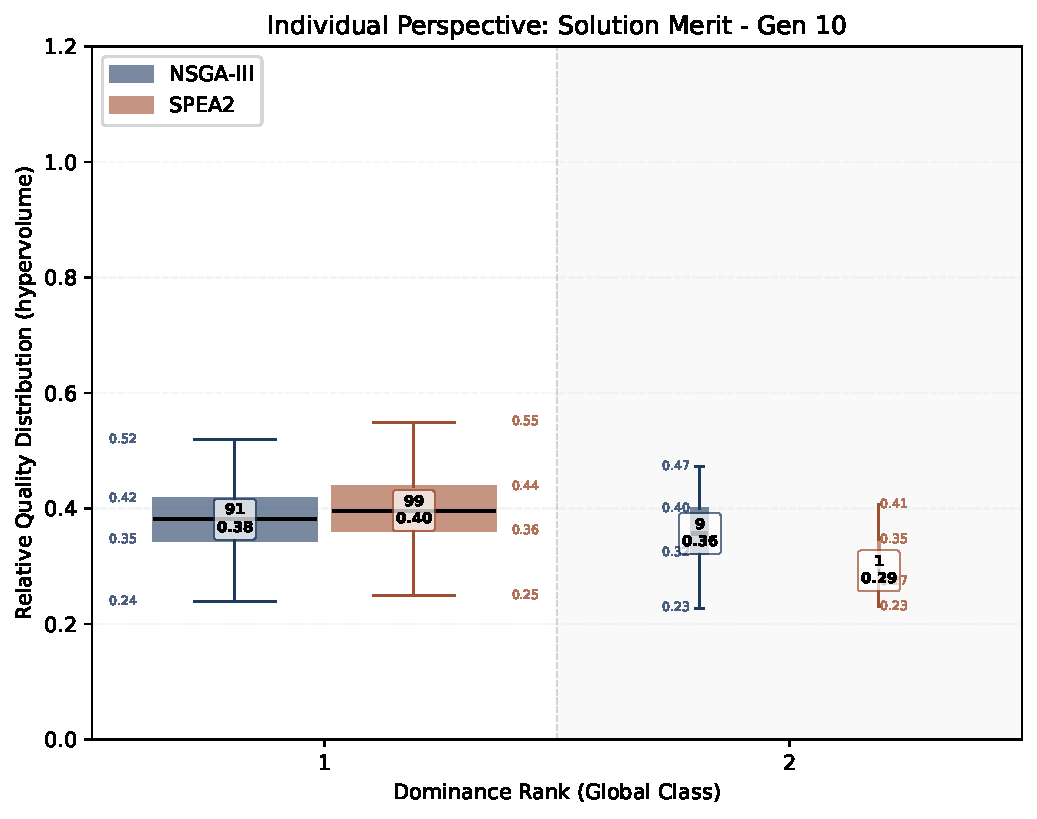
\includegraphics[width=\linewidth,height=.61\textheight,keepaspectratio]{figures/example_08_01_strata.pdf}
\end{column}
\begin{column}{.33\textwidth}
\begin{lstlisting}[style=python,basicstyle=\ttfamily\fontsize{7.0}{8.6}\selectfont]
ind = mb.stats.strata(
    exp1, exp2, gen=10,
    mode='individual')
ind.report()
mb.view.strata(ind)
\end{lstlisting}
\textbf{Rank 1 por execução:}
\par NSGA-III: \textbf{91} soluções
\par SPEA2: \textbf{99} soluções
\par\smallskip
\textbf{Mediana de mérito:}
\par 0,3811 versus 0,3962
\end{column}
\end{columns}
\vspace{.04cm}\textbf{Como ler:} o mérito é o HV dominado por cada solução isoladamente; caixas mostram a distribuição. Nessa geração, SPEA2 tem mais soluções no rank 1 e mediana individual um pouco maior.
\end{frame}

\begin{frame}[fragile]{Exemplo 8 — Strata collective: qualidade da frente como conjunto}
\begin{columns}[T,onlytextwidth]
\begin{column}{.64\textwidth}
\centering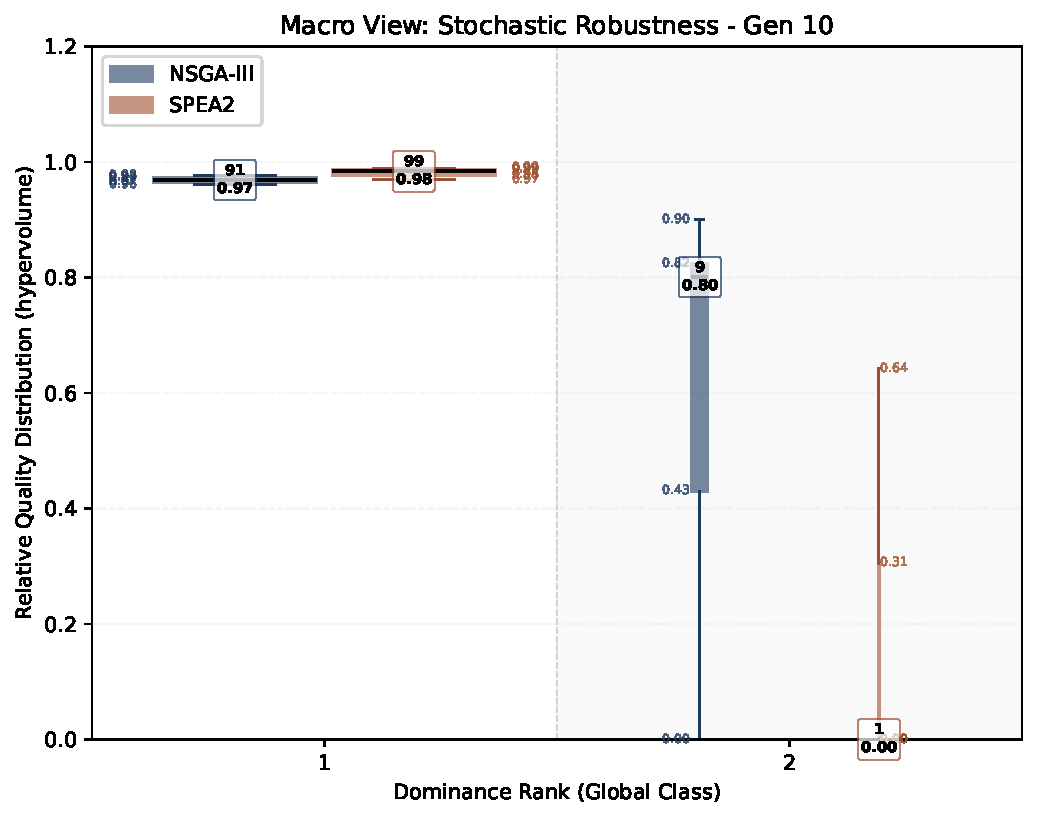
\includegraphics[width=\linewidth,height=.61\textheight,keepaspectratio]{figures/example_08_02_strata.pdf}
\end{column}
\begin{column}{.34\textwidth}
\begin{lstlisting}[style=python,basicstyle=\ttfamily\fontsize{7.0}{8.6}\selectfont]
coll = mb.stats.strata(
    exp1, exp2, gen=10,
    mode='collective')
coll.report()
mb.view.strata(coll)
\end{lstlisting}
\textbf{Mediana do HV do rank 1:}
\par NSGA-III: \textbf{0,9687}
\par SPEA2: \textbf{0,9837}
\end{column}
\end{columns}
\vspace{.04cm}\textbf{Diferença:} o modo individual mede cada ponto; o coletivo mede o \emph{conjunto de soluções} de cada rank. Pontos que isoladamente parecem modestos podem, juntos, cobrir bem a frente.
\end{frame}

\begin{frame}[fragile]{Exemplo 8 — Tiers: e se as populações competirem juntas?}
\begin{columns}[T,onlytextwidth]
\begin{column}{.66\textwidth}
\centering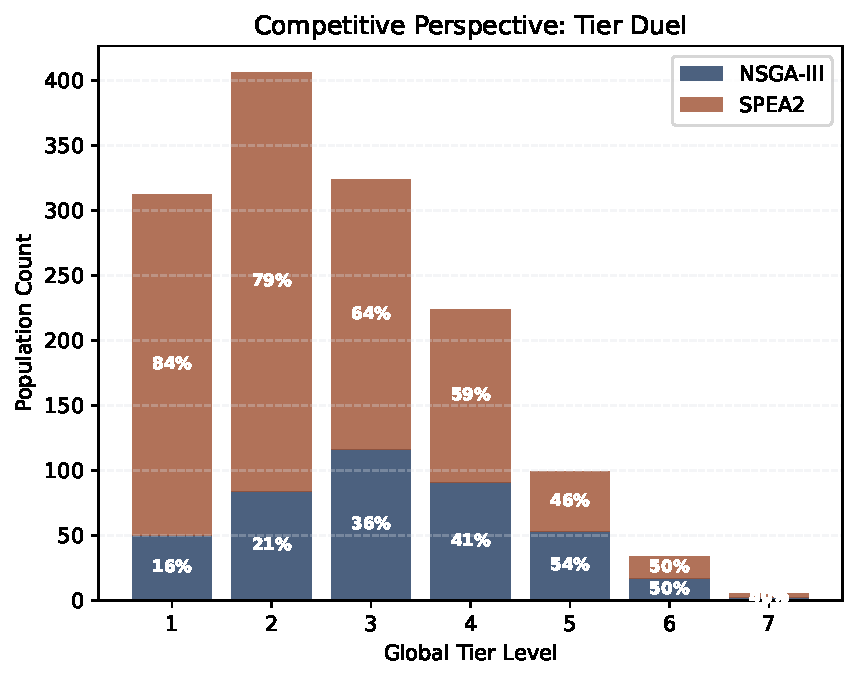
\includegraphics[width=\linewidth,height=.61\textheight,keepaspectratio]{figures/example_08_03_tiers.pdf}
\end{column}
\begin{column}{.32\textwidth}
\begin{lstlisting}[style=python,basicstyle=\ttfamily\fontsize{7.4}{9.2}\selectfont]
tiers = mb.stats.tiers(
    exp1, exp2, gen=10)
tiers.report()
mb.view.tiers(tiers)
\end{lstlisting}
\textbf{Primeiro rank global:}
\par SPEA2: \textbf{84\%}
\par NSGA-III: \textbf{16\%}
\par\smallskip
A análise constrói \textbf{sete ranks globais}.
\end{column}
\end{columns}
\vspace{.04cm}\textbf{Interpretação:} quando as soluções dos dois MOEAs são reunidas e a dominância é recalculada, SPEA2 ocupa a grande maioria das posições no rank 1. Isso é distinto dos ranks calculados isoladamente.
\end{frame}

